\documentclass[]{scrartcl}

\usepackage{graphicx}
\usepackage{float}

%opening
\title{Multi-Agent Systems Assignment 6}
\author{Alex Hoorn}

\begin{document}

\maketitle

\section{Monte Carlo Sampling}


\begin{figure}[H]
	\centering
	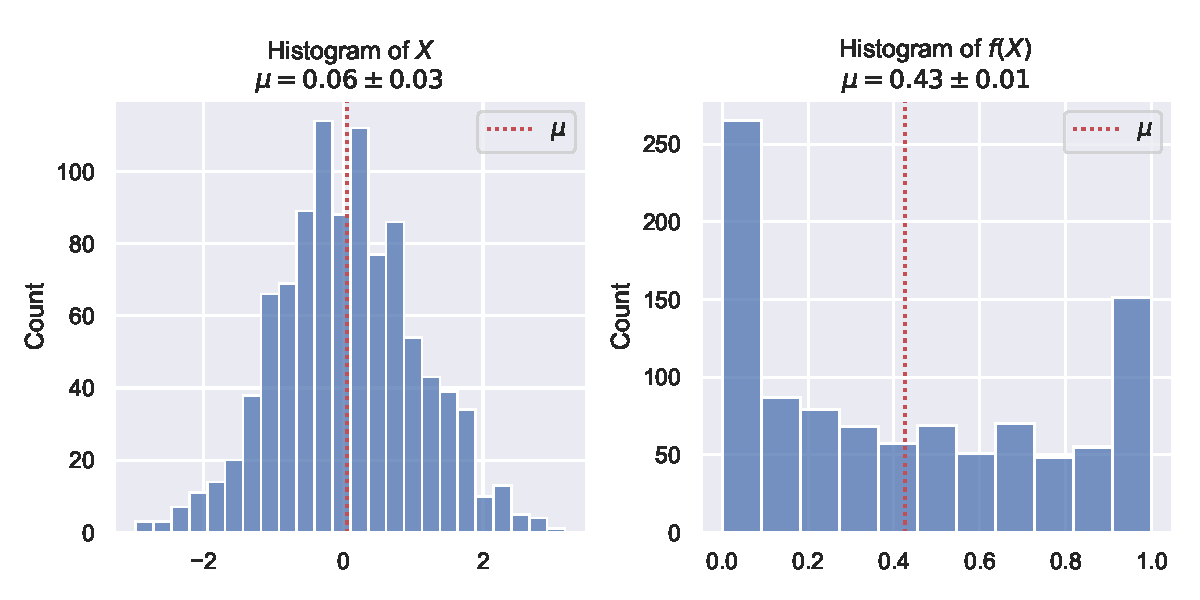
\includegraphics[width=0.7\linewidth]{1-1.pdf}
	\caption{}
	\label{fig:1-1}
\end{figure}


\begin{figure}[H]
	\centering
	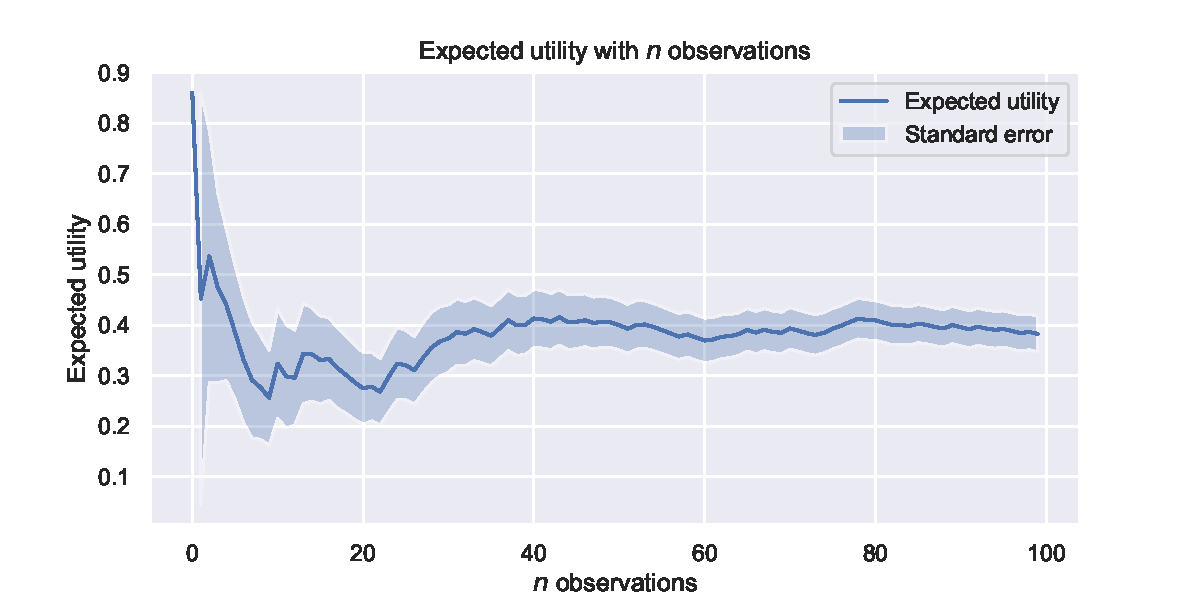
\includegraphics[width=0.7\linewidth]{1-2.pdf}
	\caption{}
	\label{fig:1-2}
\end{figure}


\section{Monte Carlo Tree Search}

\begin{figure}[H]
	\centering
	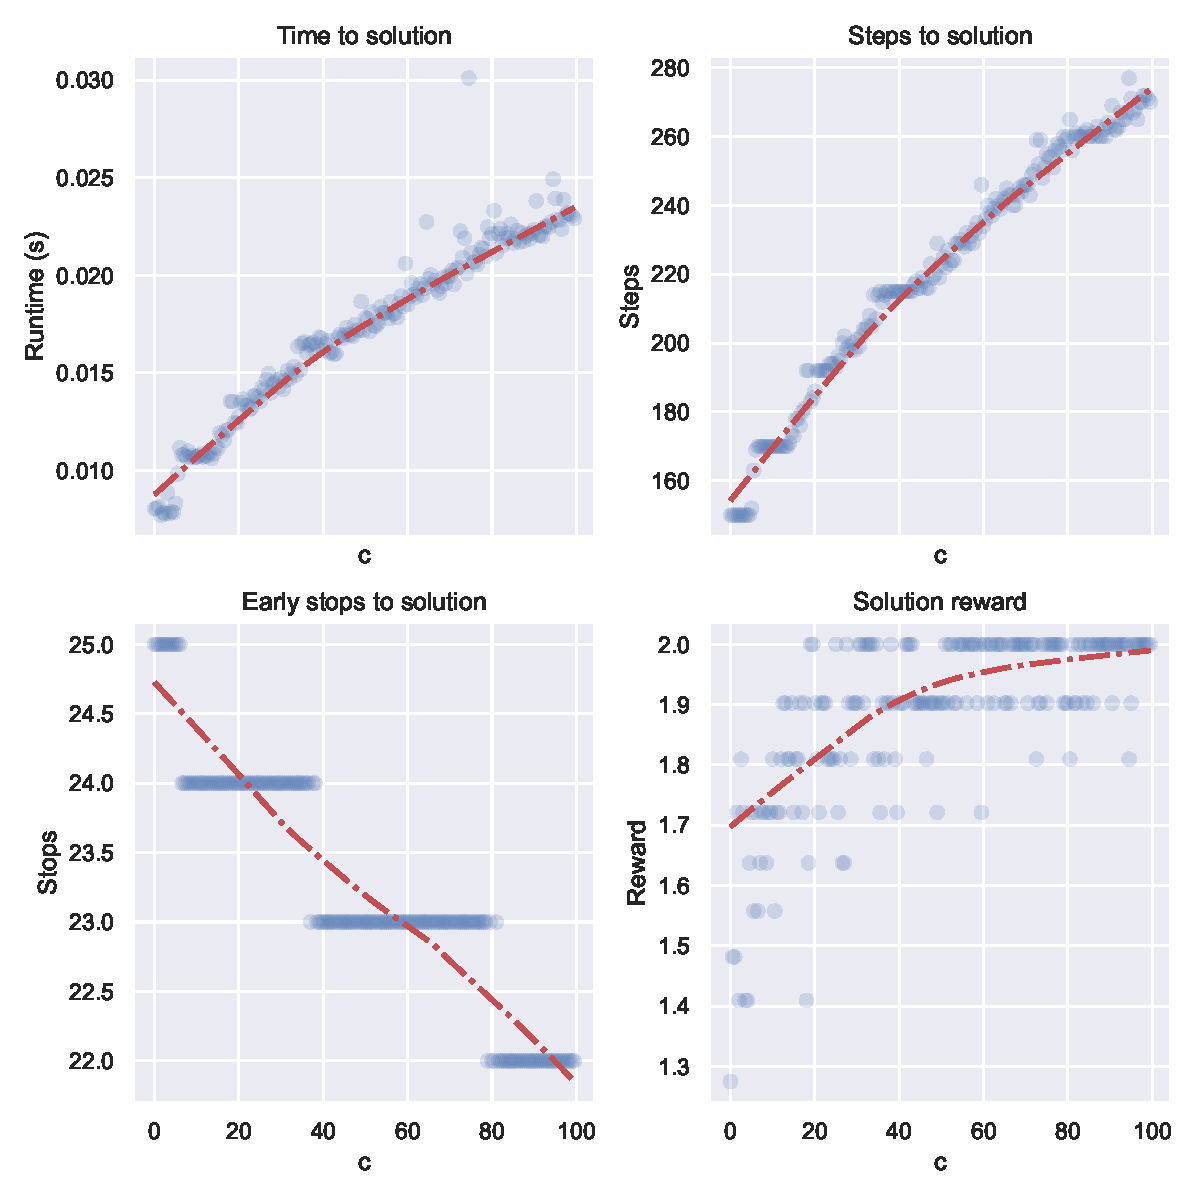
\includegraphics[width=1\linewidth]{2-1.pdf}
	\caption{}
	\label{fig:2-1}
\end{figure}


\section{Reinforcement Learning}

\end{document}
